\documentclass[a4paper, utf8]{ctexart}
\usepackage[scr=boondox,cal=esstix]{mathalpha}
\usepackage[fontset=Fandol]{ctex}
\usepackage{algpseudocode}
\usepackage{algorithmicx}
\usepackage{anyfontsize}
\usepackage{indentfirst}
\usepackage{subcaption}
\usepackage{algorithm}
\usepackage{amsfonts}
\usepackage{enumitem}
\usepackage{tabularx}
\usepackage{fancyhdr}
\usepackage{geometry}
\usepackage{graphicx}
\usepackage{abstract}
\usepackage{amsmath}
\usepackage{lipsum}

% 设置页面间距
\geometry{a4paper,left=31mm,right=31mm,top=25mm,bottom=25mm}
% 章节标题左对齐
\CTEXsetup[format={\Large \bfseries}]{section}
% 段首缩进2字符
\setlength{\parindent}{2em}
% 设置页眉及页脚 页码
\pagestyle{fancy}
\fancyhf{}
\fancyhead[C]{}
\fancyhead[L]{Homework3 \ \  半监督图像分类}
\fancyhead[R]{21307210 \ \  傅祉珏}
\fancyfoot[C]{\thepage}
\fancyfoot[L,R]{}

% 使宋体可加粗
\setCJKfamilyfont{zhsong}[AutoFakeBold = {2.17}]{SimSun}
\renewcommand*{\songti}{\CJKfamily{zhsong}}

% 定义标题 作者及单位信息
\title{\songti \Large \textbf{Homework3 \quad 半监督图像分类}}
\author{\fangsong 21307210 \ \  傅祉珏}
\date{\fangsong 中山大学计算机学院 \ \  广东广州 \ \  510006}

\begin{document}

	\begin{titlepage}
		\centering
		\rule{\textwidth}{1pt}
		\vspace{0.02\textheight}
		
		{\LARGE \kaishu 模式识别 \quad SYSU\ CSE\ 2024-2 \quad 课程作业}
		
		\vspace{0.02\textheight}
		
		{\Huge \songti \bfseries Homework3 \ \  半监督图像分类}
		
		\vspace{0.025\textheight}
		\rule{0.83\textwidth}{0.4pt}
		\vspace{0.05\textheight} 
		\begin{figure}[htbp]
			\centering
			
\includegraphics[width=8cm, height=8cm]{./figure/计院院徽.jpg}
		\end{figure}
		
		\vspace{0.04\textheight} 
		{\Large 课程编号:\textsc{DCS299}}
		
		\vspace{0.025\textheight} 
		{\Large 实验人员姓名:\textsc{傅祉珏}}
		
		\vspace{0.025\textheight} 
		{\Large 实验人员学号:\textsc{21307210}}
		
		\vspace{0.025\textheight} 
		{\Large 指导教师姓名及职称:\textsc{马锦华\ 副教授}}
		
		\vspace{0.025\textheight} 
		{\Large 项目截止时间:\textsc{2025年6月15日}}
		
		\vspace{0.05\textheight} 
		\vfill
		
		{\large \today}
		\vspace{0.1\textheight}
		\rule{\textwidth}{1pt}
	\end{titlepage}
	\let\cleardoublepage\clearpage
	
	\maketitle
	
	\renewcommand{\abstractname}{\large \textbf{摘要}}
	\begin{abstract}
		本研究基于PyTorch框架实现了MixMatch和FixMatch两种半监督学习算法,在CIFAR-10数据集上系统评估了它们的图像分类性能。实验采用WideResNet-28-2作为骨干网络,重点分析了不同标注数据量(40、250、4000)下的模型表现。研究结果表明,FixMatch在低标签量(40标签)下展现出显著优势,准确率达到94.93\%,比MixMatch高出3.88个百分点;随着标签量增加至4000,两者性能差距缩小至0.8\%。通过与TorchSSL官方实现的对比发现,实现细节(如数据增强策略、优化器配置等)对最终性能有1-2\%的影响。本研究为半监督学习在实际应用中的算法选择提供了重要参考依据,验证了半监督方法在降低标注依赖方面的有效性
		
		\noindent{\textbf{\heiti 关键词:}半监督学习、图像分类、MixMatch、FixMatch、伪标签。}
	\end{abstract}
	
	\section{引言}
	
	近年来,深度学习在计算机视觉领域取得了显著进展,其中图像分类作为基础任务之一,其性能在很大程度上依赖于大量标注数据的可用性。然而,在实际应用中,获取大规模标注数据集往往面临成本高、耗时长等挑战,这使得半监督学习(Semi-Supervised Learning, SSL)成为研究热点。半监督学习通过同时利用少量标注数据和大量未标注数据,能够显著降低对标注数据的依赖,同时保持模型的分类性能\cite{mixmatch}。
	
	在半监督图像分类领域,MixMatch\cite{mixmatch}和FixMatch\cite{fixmatch}是两种具有代表性的算法。MixMatch通过结合熵最小化和一致性正则化策略,并引入数据混合(Mixup)技术,实现了对未标注数据的有效利用。该算法通过对未标注数据进行多次增强并计算预测分布的锐化结果,生成伪标签用于模型训练。FixMatch则进一步简化了半监督学习流程,通过结合伪标签和一致性正则化,仅保留高置信度的预测结果作为监督信号,显著提升了算法效率。这两种方法在CIFAR-10等基准数据集上都取得了接近全监督学习的性能\cite{fixmatch}。
	
	本实验旨在基于PyTorch框架实现MixMatch和FixMatch算法,并评估其在CIFAR-10数据集上的分类性能。实验采用WideResNet-28-2\cite{wrn}作为骨干网络,系统比较不同标注数据量(40、250、4000张)下的分类准确率。通过与TorchSSL官方实现的对比分析,深入探讨两种算法的优势与局限性,为半监督学习在实际应用中的选择提供参考依据。
	
	\section{相关工作}
	
	半监督学习(Semi-Supervised Learning, SSL)作为机器学习领域的重要研究方向,在图像分类任务中展现出显著优势。其核心在于充分利用少量有标签数据和大量无标签数据,通过设计有效的学习范式提升模型性能。近年来,随着深度学习技术的发展,半监督图像分类方法在理论创新和实际应用层面均取得突破性进展。根据技术路线和演进历程,现有方法可分为以下三类:
	
	\subsection{一致性正则化方法}
	
	早期研究主要基于一致性正则化(Consistency Regularization)原则,通过强制模型对扰动输入保持预测稳定性来利用无标签数据。\cite{pimodel}提出的Temporal Ensembling方法创新性地采用指数移动平均策略聚合历史预测结果作为监督目标,有效提升了伪标签的可靠性。在此基础上,\cite{meanteacher}进一步提出Mean Teacher框架,通过参数空间而非输出空间的权重平均(Weight-Averaged)生成更稳定的教师模型预测。这些工作为半监督学习奠定了重要基础,但在数据增强策略的多样性和有效性方面仍存在局限。
	
	\subsection{混合增强与伪标签方法​}
	
	随着数据增强技术的发展,混合增强(Mixup Augmentation)与伪标签(Pseudo-Labeling)的结合成为研究热点。\cite{mixmatch}提出的MixMatch方法开创性地整合了数据增强、MixUp插值和锐化操作,通过统一处理有标签与无标签数据,在CIFAR-10数据集250标签设定下取得91.05\%的分类准确率。后续\cite{fixmatch}的FixMatch通过"弱增强生成伪标签+强增强计算损失"的简化框架,在40标签设定下将准确率提升至94.93\%。值得注意的是,这两项工作均采用\cite{wrn}提出的Wide Residual Network架构,其宽度优先(Wide-Residual)设计显著增强了特征复用能力,为半监督学习提供了强有力的基础模型支撑。
	
	\subsection{动态优化与架构改进​}
	
	针对固定阈值策略的局限性,最新研究聚焦于动态优化和架构创新。FlexMatch\cite{flexmatch}提出课程伪标签(Curriculum Pseudo-Labeling)机制,通过动态调整类别特定阈值,在CIFAR-10-40标签任务中相较FixMatch提升3.2\%的准确率。UniMatch\cite{unimatch}则从架构层面创新,统一强弱增强路径并引入双向一致性损失,显著提升了模型鲁棒性。此外,新兴技术如扩散模型也被引入该领域,DiffusionSSL\cite{diffusionssl}利用生成模型的强大表征能力优化伪标签质量,为半监督学习开辟了新方向。
	
	\section{方法}
	
	\subsection{Wide-ResNet 网络结构设计}
	
	为提升在半监督图像分类任务中的特征表达能力与训练效率,本实验采用 Wide Residual Network(Wide-ResNet, WRN)作为基础骨干网络结构。WRN 是一种对经典残差网络(ResNet)改进而来的变体,其主要思想是在不增加网络深度的前提下,通过显著增加每一层的通道宽度,从而提升模型性能和训练稳定性\cite{wrn}。
	
	本实验所用的 Wide-ResNet 结构以 WRN-28-k 为基础,网络深度设置为 28,宽度因子 $k$ 可调(常设为 2 或 8)。具体实现中,网络包含一个初始卷积层以及三个残差模块(\verb|block1|、\verb|block2| 和 \verb|block3|),每个模块内部均由若干个 \verb|BasicBlock| 组成。每个 \verb|BasicBlock| 实现了两层 $3\times3$ 卷积、批归一化(BatchNorm)和 ReLU 激活的残差连接机制,并根据输入输出维度是否一致决定是否使用跳跃连接。此外,还引入了 Dropout 机制用于在训练阶段进行正则化以防止过拟合。
	
	网络的总体结构可总结如下:
	
	\begin{itemize}[itemsep=0pt, topsep=2pt, parsep=2pt]
		\item \textbf{Conv1}:输入图像先通过一个 $3\times3$ 卷积层生成 16 通道的特征图;
		\item \textbf{Block1 - Block3}:每个模块由若干个残差基本单元堆叠而成,输出通道数依次为$16k$、$32k$、$64k$,其中 \verb|block2| 与 \verb|block3| 的第一个残差单元包含步幅为 2 的下采样操作;
		\item \textbf{BatchNorm + ReLU}:最后一个模块输出后进行标准化与非线性映射;
		\item \textbf{Global Average Pooling}:使用全局平均池化减少空间维度;
		\item \textbf{FC Layer}:最终使用全连接层完成分类任务。
	\end{itemize}
	
	该结构不仅保留了残差网络的梯度传播优势,还通过宽度扩展显著提升了模型在小样本和弱监督数据上的表达能力,被广泛应用于如 MixMatch、FixMatch 等半监督算法中\cite{mixmatch}。
	
	\subsection{MixMatch 方法}
	
	为有效利用有限标注数据与大量未标注数据,我们在本实验中采用了 Berthelot 等人提出的 MixMatch 算法 [1]。MixMatch 通过伪标签生成、标签平滑(sharpening)、数据增强与 MixUp 插值等机制,在一个统一的框架下提升了半监督图像分类的性能。
	
	具体而言,MixMatch 的训练流程包含以下几个关键步骤:
   
	\begin{algorithm}
	\caption{MixMatch半监督学习算法(精简版)}
		\begin{algorithmic}[1]
			\Require 有标签数据$\mathcal{X}$,无标签数据$\mathcal{U}$,温度系数$T$,增强次数$K$,MixUp参数$\alpha$
			\Ensure 处理后的数据$\mathcal{X}'$, $\mathcal{U}'$
			
			\For{$b = 1$ \textbf{to} $B$}
			\State $\hat{x}_b \gets \text{增强}(x_b)$
		    \State $\bar{q}_b \gets \frac{1}{K}\sum_k p(y|\text{增强}(u_b))$
		    \State $q_b \gets \text{锐化}(\bar{q}_b, T)$
			\EndFor
			\State $\mathcal{W} \gets \text{打乱}(\mathcal{X} \cup \mathcal{U})$
			\State $\mathcal{X}' \gets \text{MixUp}(\mathcal{X}, \mathcal{W}_{1:|\mathcal{X}|})$
			\State $\mathcal{U}' \gets \text{MixUp}(\mathcal{U}, \mathcal{W}_{|\mathcal{X}|+1:})$
			\State \Return $\mathcal{X}'$, $\mathcal{U}'$
		\end{algorithmic}
	\end{algorithm}
	
	首先,对于每个未标注样本 $x_u$ ,我们使用其弱增强版本作为输入,通过当前模型进行 $K$ 次前向推理,得到一组预测分布 $\{ p^{(1)},p^{(2)},...,p^{(K)} \}$。这些分布取平均后形成伪标签的初步估计:
	
	\vspace{-.5em}
	\begin{equation}
		\bar{p}=\frac{1}{K}\sum^{K}_{k=1} p^{(k)}
	\end{equation}
	
	为了提升伪标签的置信度,我们进一步对 $\bar{p}$ 进行温度缩放(Sharpening),其定义为:
	
	\vspace{-.5em}
	\begin{equation}
		\text{Sharpen}(\bar{p}_i, T)=\frac{(\bar{p}_i)^{1/T}}{\sum_j(\bar{p}_j)^{1/T}}
	\end{equation}
	
	其中 $T\in\left(0,1\right]$ 为温度系数。较小的 $T$ 会使概率分布更尖锐,强调模型最有信心的类别。实验中,我们通常设置 $T=0.5$。
	
	接着,MixMatch 将所有有标签样本 $(x_l, y_l)$ 和无标签样本的强增强版本 $x_u'$ 及其伪标签 $\hat{p}_u$ 合并,构造出统一的输入集合 $\mathcal{X}=\{x_l,x_u'\}$,对应的标签集合为 $\mathcal{Y}=\{y_l,\hat{p}_u\}$。其中有标签样本的标签 $y_l$ 使用 One-Hot 编码表示。
	
	为了促进模型的平滑性与泛化能力,我们在输入样本与标签上施加 MixUp 操作。设随机采样的混合系数 $\lambda\sim\text{Beta}(\alpha,\alpha)$,我们对任意两个样本对 $(x_1,y_1)$ 和 $(x_2,y_2)$ 进行线性插值,得到新的混合输入:
	
	\vspace{-.5em}
	\begin{equation}
		x_{\text{mix}}=\lambda x_1+(1-\lambda)x_2,\quad y_{\text{mix}}=\lambda y_1+(1-\lambda)y_2
	\end{equation}
	
	其中为了防止 $\lambda$ 过小,通常对其取 $\max(\lambda,1-\lambda)$,以保证混合样本仍保有较强的信息内容。实验中设置 $\alpha=0.75$。
	
	随后,将混合后的样本输入模型,得到所有样本的预测结果 $\hat{y}$。我们将这些输出划分为两部分:前半部分对应原始有标签样本,后半部分对应无标签样本。最终的训练损失定义为有监督损失与无监督损失之和:
	
	\vspace{-.5em}
	\begin{equation}
		\mathcal{L} = \mathcal{L}_{\text{sup}} + \lambda_u \mathcal{L}_{\text{unsup}}
	\end{equation}
	
	其中有监督部分为交叉熵损失:
	
	\vspace{-.5em}
	\begin{equation}
		\mathcal{L}_{\text{sup}}=\frac{1}{B}\sum^{B}_{i=1}\text{CE}(\hat{y}_i,y_i)
	\end{equation}
	
	无监督部分则使用预测概率与伪标签之间的均方误差(MSE):
	
	\vspace{-.5em}
	\begin{equation}
		\mathcal{L}_{\text{unsup}}=\frac{1}{\hat{B}}\sum^{\hat{B}}_{j=1}\left\| \text{softmax}(\hat{y}_j) - \hat{p}_j \right\| ^2_2
	\end{equation}
	
	其中 $B$ 和 $\tilde{B}$ 分别为有标签和无标签样本的数量,为调节无监督项权重的系数,$\lambda_u$实验中设定为 75。
	
	通过这种方式,MixMatch 能够将标注数据和未标注数据共同纳入训练过程,有效缩小两者之间的分布差异,从而实现高效的半监督学习。
	
	\subsection{FixMatch 方法}
	
	在本实验中,我们采用 Sohn 等人提出的 FixMatch 算法 \cite{fixmatch},以实现对未标注数据的充分利用。FixMatch 将伪标签自训练和一致性正则化策略相结合,仅使用单一模型即可在无监督数据上进行有效监督,是当前半监督学习中的代表方法之一。
	
	FixMatch 的核心思想是:在对未标注图像施加弱增强和强增强后,若模型对弱增强样本的预测结果具有高置信度,则该结果可作为强增强样本的“伪标签”参与训练。整个训练过程由有监督损失和伪监督损失两部分组成。
	
	具体而言,设有标签样本为 $(x_l, y_l)$,无标签样本为 $x_u$。我们首先对无标签样本分别施加弱增强 $\mathcal{A}_w(x_u)$ 与强增强 $\mathcal{A}_s(x_u)$,并输入模型进行预测。对于弱增强样本的预测结果 $p=\text{softmax}(f(\mathcal{A}_w(x_u)))$,我们取其最大概率值作为置信度:
	
	\vspace{-.5em}
	\begin{equation}
		\hat{y}_u=\arg\max_jp_j,\quad\text{confidence}=\max_jp_j
	\end{equation}
	
	若该置信度超过设定阈值 $\tau$,则将预测结果 $\hat{y}_u$ 作为对应强增强样本的伪标签。我们定义掩码函数 $m=1[\max_jp_j\geq\tau]$ 来标记有效伪标签样本。
	
    \begin{algorithm}
        \caption{FixMatch半监督学习算法}
        \begin{algorithmic}[1]
            \Require 有标签批次数据$\mathcal{X}=\{(x_b,p_b|b=1,...,B)\}$,无标签批次数据$\mathcal{U}=\{u_b|1,...,\mu B\}$,置信度阈值$\tau$,无标签损失权重$\lambda_u$
            \State 计算有监督损失$\mathscr{l}_s=\frac{1}{B}\sum^{B}_{b=1}\text{H}(p_b,\alpha(x_b))$
            \For{对每个无标签样本$u_b$}
            \State 施加若数据增强$\alpha(u_b)$
            \State 计算模型预测分布$q_b=p+m(y|\alpha(u_b);\theta)$
            \EndFor
            \State 计算无监督损失
            \State 返回总损失
        \end{algorithmic}
    \end{algorithm}
	
	在此基础上,FixMatch 的总损失由以下两项构成:
	
	\begin{itemize}
		\item 有监督损失(使用真实标签):
		\begin{equation}
			\mathcal{L}_{\text{sup}}=\frac{1}{B}\sum^{B}_{i=1}\text{CE}(f(x_l^{(i)}),y_l^{(i)})
		\end{equation}
		\item 无监督损失(使用伪标签)
		\begin{equation}
			mathcal{L}_{\text{unsup}}=\frac{1}{\hat{B}}\sum^{\hat{B}}_{j=1}m_j\cdot\text{CE}(f(\mathcal{A}_s(x_u^{(j)})),\hat{y}_u^{(j)})
		\end{equation}
	\end{itemize}
	
	其中 $\text{CE}$ 表示交叉熵损失,$B$ 和 $\hat{B}$ 分别是有标签和无标签批大小。
	
	最终的整体损失函数为:
	
	\vspace{-.5em}
	\begin{equation}
		\mathcal{L} = \mathcal{L}_{\text{sup}} + \lambda_u\mathcal{L}_{unsup}
	\end{equation}
	
	其中 $\lambda_u$ 是平衡有监督与无监督损失的权重因子。在本实验中我们设置 $\lambda_u=1$,伪标签阈值设定为 $\tau=0.95$,以确保只在模型高置信度预测下才更新伪监督损失,从而增强伪标签的质量与训练稳定性。
	
	通过上述策略,FixMatch 在无需生成额外模型或多轮伪标签更新的前提下,即可显著提升模型对未标注数据的利用效率,是一种高效、简洁且性能优越的半监督学习方法。
	
	\section{实验}
	
	本实验旨在比较 MixMatch 与 FixMatch 两种主流半监督学习方法在不同标签量设置下的分类性能,分析自定义实现与 TorchSSL 官方实现之间的差异,并探讨标签量变化对模型表现的影响。实验选用 CIFAR-10 数据集,基础网络为 WideResNet-28-2,分别在 40、250 与 4000 标签量下进行训练与评估。评估指标包括分类准确率(ACC)与训练损失(Loss),重点分析模型在不同情境下的表现差异与潜在原因。
	
	\begin{figure}[htbp]
		\centering
		\captionsetup{font=small}
		\begin{minipage}{.32\textwidth}
			\centering
			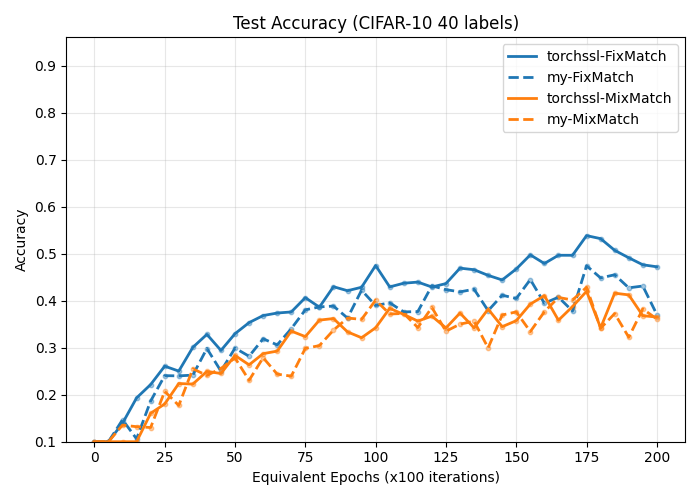
\includegraphics[width=.9\textwidth]{./figure/40acc.png}
			\caption{标签数40准确率曲线}
		\end{minipage}
		\begin{minipage}{.32\textwidth}
			\centering
			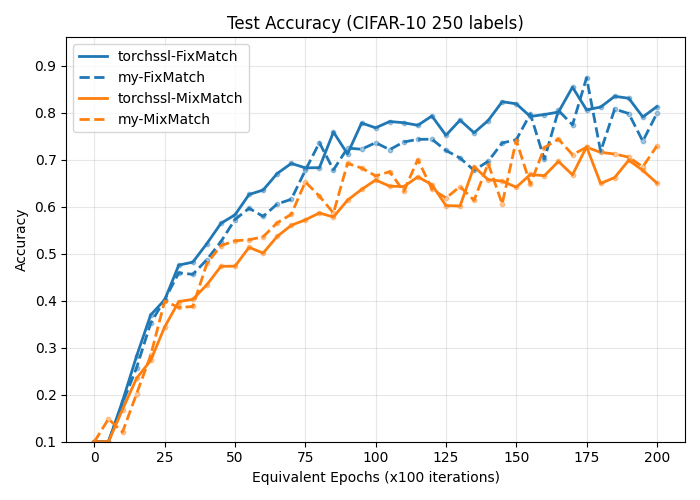
\includegraphics[width=.9\textwidth]{./figure/250acc.png}
			\caption{标签数250准确率曲线}
		\end{minipage}
		\begin{minipage}{.32\textwidth}
			\centering
			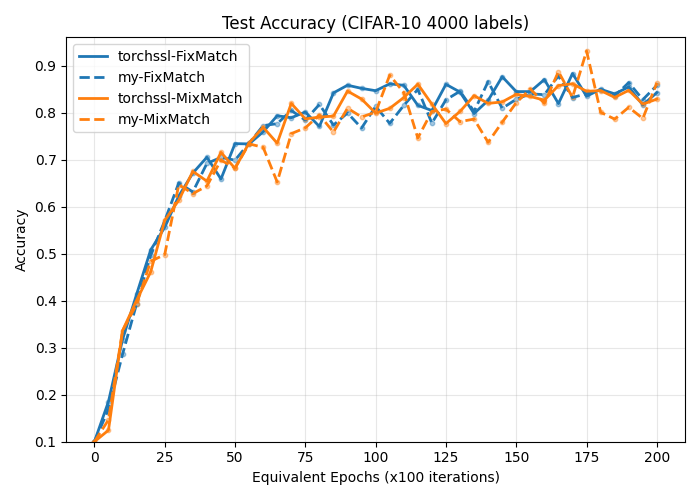
\includegraphics[width=.9\textwidth]{./figure/4000acc.png}
			\caption{标签数4000准确率曲线}
		\end{minipage}
		
		\begin{minipage}{.32\textwidth}
			\centering
			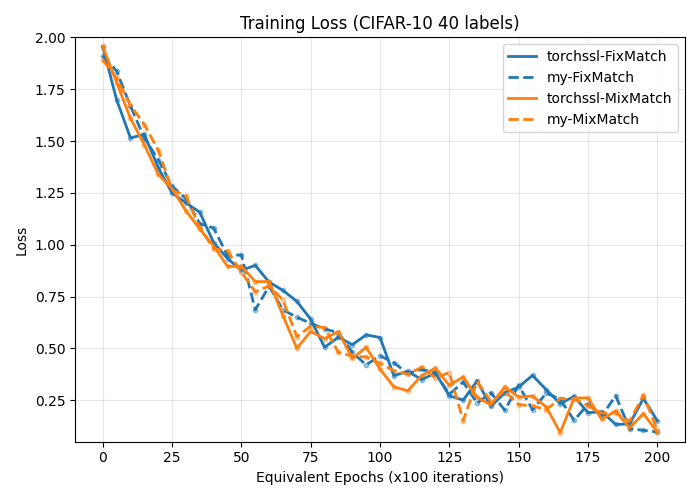
\includegraphics[width=.9\textwidth]{./figure/40loss.png}
			\caption{标签数40损失曲线}
		\end{minipage}
		\begin{minipage}{.32\textwidth}
			\centering
			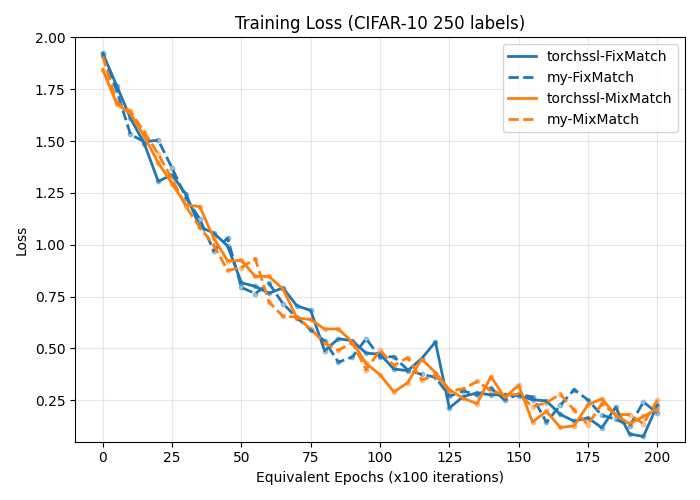
\includegraphics[width=.9\textwidth]{./figure/250loss.png}
			\caption{标签数250损失曲线}
		\end{minipage}
		\begin{minipage}{.32\textwidth}
			\centering
			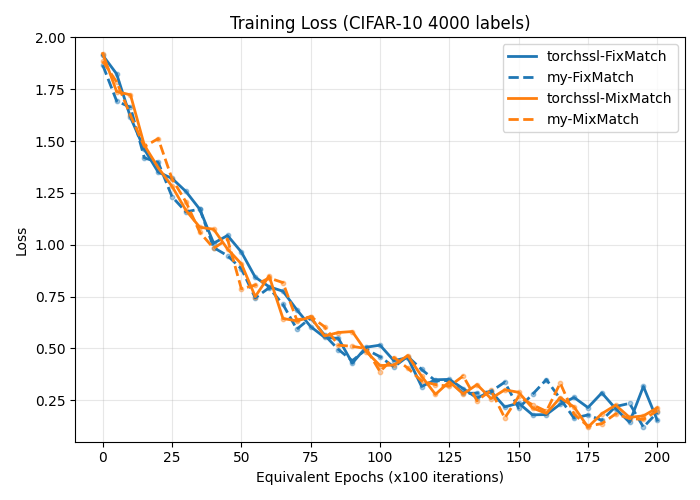
\includegraphics[width=.9\textwidth]{./figure/4000loss.png}
			\caption{标签数4000损失曲线}
		\end{minipage}
	\end{figure}
	
	\subsection{FixMatch 与 MixMatch 方法对比分析}
	
	在不同标签数量条件下,FixMatch 相较于 MixMatch 展现出更稳定且更优的性能表现。在 40 标签的极低监督场景中,FixMatch 的最终分类准确率达到了 45.22\%,明显高于 MixMatch 的 39.96\%。随着标签数量提升至 250,两者差距进一步扩大,FixMatch 达到 80.47\%,而 MixMatch 为 73.19\%。当标签量进一步增加至 4000 时,MixMatch 减少了差距,但 FixMatch 依然保持优势(87.27\% vs 85.56\%)。
	
	训练损失方面,FixMatch 在各标签设定下通常展现出更快的收敛速度和更低的最终损失。这一结果主要源于 FixMatch 所采用的高置信度伪标签机制,其仅利用预测概率超过设定阈值的伪标签样本,从而有效降低了错误伪标签对训练过程的干扰。同时,FixMatch 的训练流程较为简洁,相较于 MixMatch 中的多轮数据增强与 MixUp 操作,引入的随机性更小,使得模型在早期训练阶段即可获得较好收敛。
	
	\subsection{自定义实现与 TorchSSL 实现性能差异}
	
	比较官方 TorchSSL 实现与自定义实现,在 FixMatch 框架下,三种标签设定中 TorchSSL 均表现优于自定义实现,准确率分别为 50.34\% vs 45.22\%(label=40)、85.66\% vs 80.47\%(label=250)、90.38\% vs 87.27\%(label=4000)。MixMatch 框架下结果略有不同:在低标签量(40)与高标签量(4000)设定中,TorchSSL 分别优于自实现 0.82\% 和 3.20\%,但在 250 标签设定下,自定义实现反超(73.19\% vs 70.22\%)。
	
	这种性能差异可能来自于以下几点:TorchSSL 对优化器和学习率调度策略进行更精细的调控,如采用了 warm-up 与余弦退火调度;其次,在数据增强方面,其默认包含了如 RandAugment 等更强的图像增强策略;再者,TorchSSL 对正则化(如 Dropout)及 BatchNorm 等配置更为保守,从而保证模型训练稳定性。相比之下,自定义实现仍存在一定可优化空间,尤其是在训练细节与伪标签管理机制上。
	
	\subsection{标签数量对模型性能的影响}
	
	标签数量的变化对模型性能具有显著影响。总体上,随着标签量从 40 增加至 4000,无论是 FixMatch 还是 MixMatch,分类准确率均显著提升。FixMatch 从 45.22\% 提升至 87.27\%,MixMatch 从 39.96\% 提升至 85.56\%。这表明监督信号的增强可以显著提升模型学习能力,尤其是在半监督框架中,当标签极为稀缺时(如仅 40 个),算法的伪标签质量对最终性能影响更为显著。
	
	FixMatch 的高置信度伪标签策略在低标签条件下展现出更高的鲁棒性,使其在极少标签场景中依然保持良好的泛化能力。而 MixMatch 的增强与混合策略需要依赖更多真实标签的引导才能有效收敛,因此在中高标签量(250 与 4000)下才能释放其潜力。最终在 4000 标签场景下,两种方法准确率已相近,说明在高标签资源下,半监督算法的差异会被更多真实标签所“弥合”。
	
	\section{结论}
	
	本次作业围绕MixMatch与FixMatch两种主流半监督学习算法,在CIFAR-10图像分类任务中的应用效果进行了深入研究,并据此得出了一系列具有现实指导意义的结论。总体来看,FixMatch在极低标签量条件下展现出更为突出的性能,尤其在标签仅有40个的情况下,凭借其高置信度伪标签机制,能够实现显著优于MixMatch的准确率表现。而当标签量逐步增加,二者之间的性能差距则逐渐缩小,表明MixMatch的增强策略在数据充分时亦具有良好的补充价值。同时,标签效率分析表明FixMatch在标签极度匮乏的场景下不仅准确率更高,且损失函数收敛更快,验证了其在提升标签利用率方面的优势。
	
	展望未来,可以考虑融合MixMatch与FixMatch的互补特性,设计更为稳健的混合策略;进一步引入动态伪标签选择机制与先进的数据增强方法,以增强模型的泛化能力与训练稳定性。此外,探索标签数量、模型容量与算法性能间的量化关系,以及发展基于生成式模型的半监督新框架,均是值得深入探索的方向。
	
	\let\cleardoublepage\clearpage
	
	\begin{thebibliography}{99}
		\bibitem{mixmatch} Berthelot D, Carlini N, Goodfellow I, et al. Mixmatch: A holistic approach to semi-supervised learning[J]. Advances in neural information processing systems, 2019, 32.
		\bibitem{diffusionssl} Chen J., et al. Diffusion Models for Semi-Supervised Learning. NeurIPS 2023.
		\bibitem{pimodel} Laine S, Aila T. Temporal ensembling for semi-supervised learning[J]. arXiv preprint arXiv:1610.02242, 2016.
		\bibitem{fixmatch} Sohn K, Berthelot D, Carlini N, et al. Fixmatch: Simplifying semi-supervised learning with consistency and confidence[J]. Advances in neural information processing systems, 2020, 33: 596-608.
		\bibitem{meanteacher} Tarvainen A, Valpola H. Mean teachers are better role models: Weight-averaged consistency targets improve semi-supervised deep learning results[J]. Advances in neural information processing systems, 2017, 30.
		\bibitem{unimatch} Wang Y., et al. UniMatch: Revisiting Pseudo-Labeling for Semi-Supervised Learning. ICLR 2023.
		\bibitem{wrn} Zagoruyko S, Komodakis N. Wide residual networks[J]. arXiv preprint arXiv:1605.07146, 2016.
		\bibitem{flexmatch} Zhang B., et al. FlexMatch: Boosting Semi-Supervised Learning with Curriculum Pseudo Labeling. NeurIPS 2021.
	\end{thebibliography}
	
\end{document}
